\section{Data-Driven Alignment}

Stage commands and filename-derived coordinates describe the intended
micro-scan. They are valuable priors but cannot be used as alignment ground
truth. The reason is empirical: image-derived contour alignment gives lower
held-out contour distances than filename affine fits, and visual overlays show
that filename-based shifts are not sufficiently accurate for the SR forward
model.

\begin{figure}[t]
\centering
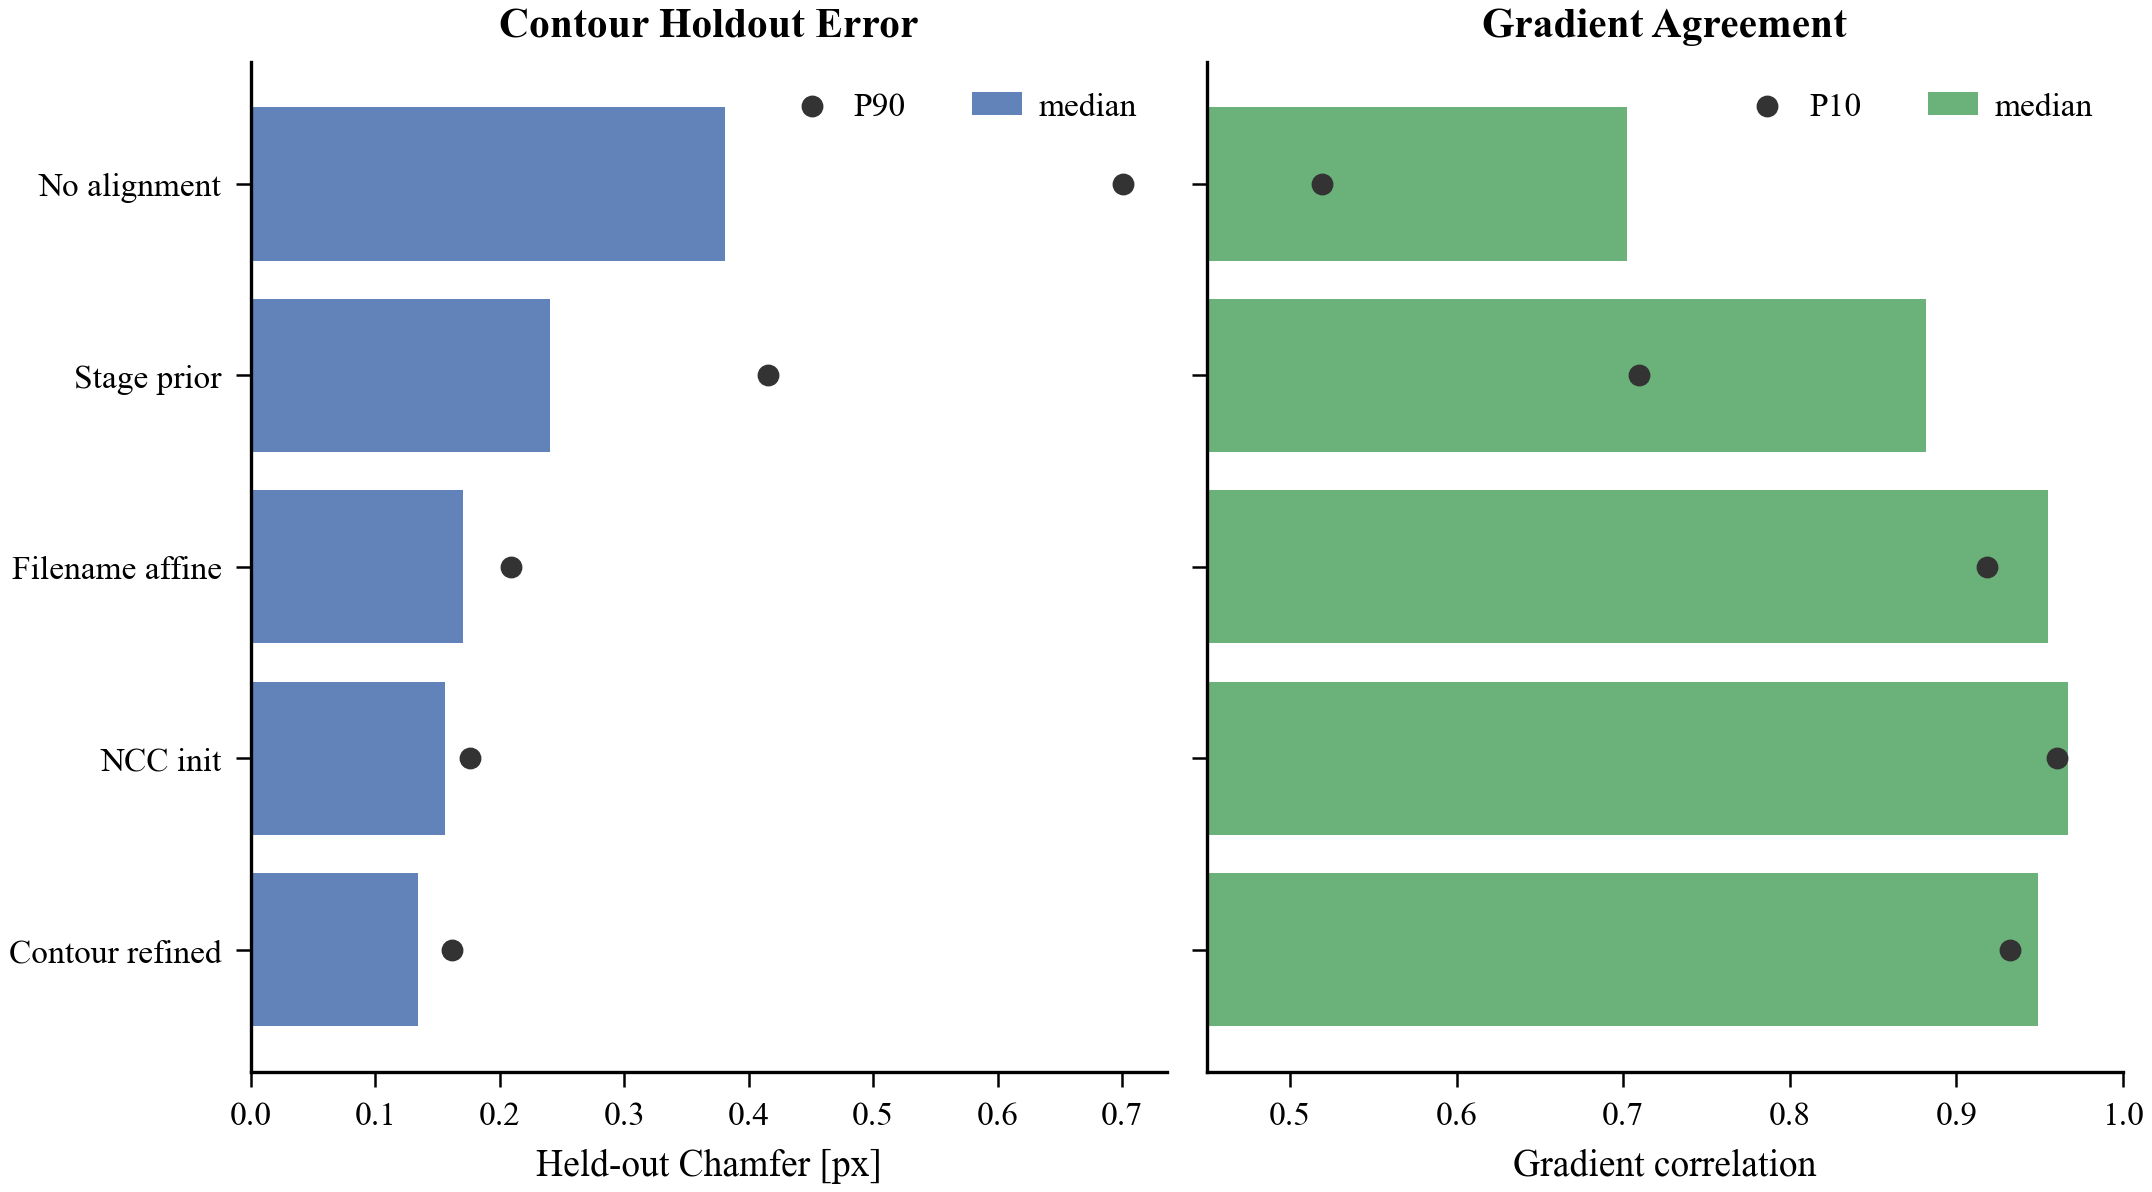
\includegraphics[width=\linewidth]{../figures/ep05_alignment_methods.png}
\caption{Alignment method comparison. Filename and stage priors are controls;
data-driven contour alignment is the SR alignment candidate.}
\label{fig:alignment-methods}
\end{figure}

The alignment pipeline uses NCC initialization followed by contour-refined
alignment against a selected reference frame. EP05 tuning further evaluates
edge thresholds, refinement radii, and subpixel steps. The tuned refined
variant improves held-out Chamfer in EP05, but EP06 shows that this does not
automatically improve split-half stability or forward-model behavior.

\begin{figure}[t]
\centering
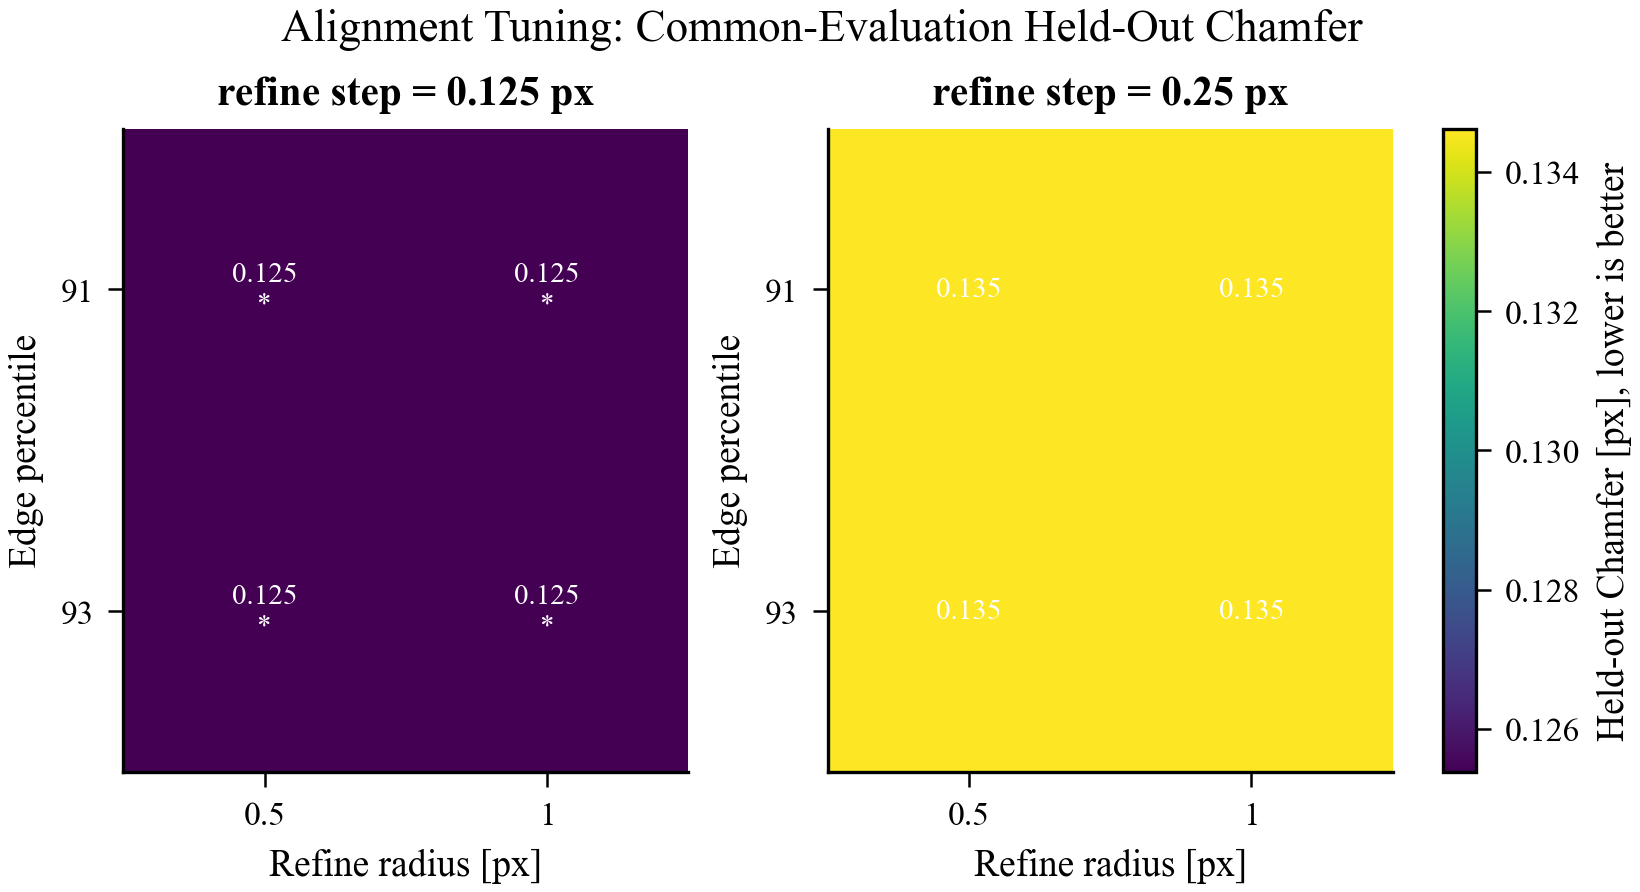
\includegraphics[width=\linewidth]{../figures/ep05_alignment_tuning_heatmap.png}
\caption{Alignment tuning curve over candidate contour-refinement settings.
This is used as sensitivity evidence, not as an automatic final-method
selector.}
\label{fig:alignment-tuning}
\end{figure}

